\documentclass[tikz,border=2mm]{standalone}

\begin{document}
\color[rgb]{0.75 0 0}
{
	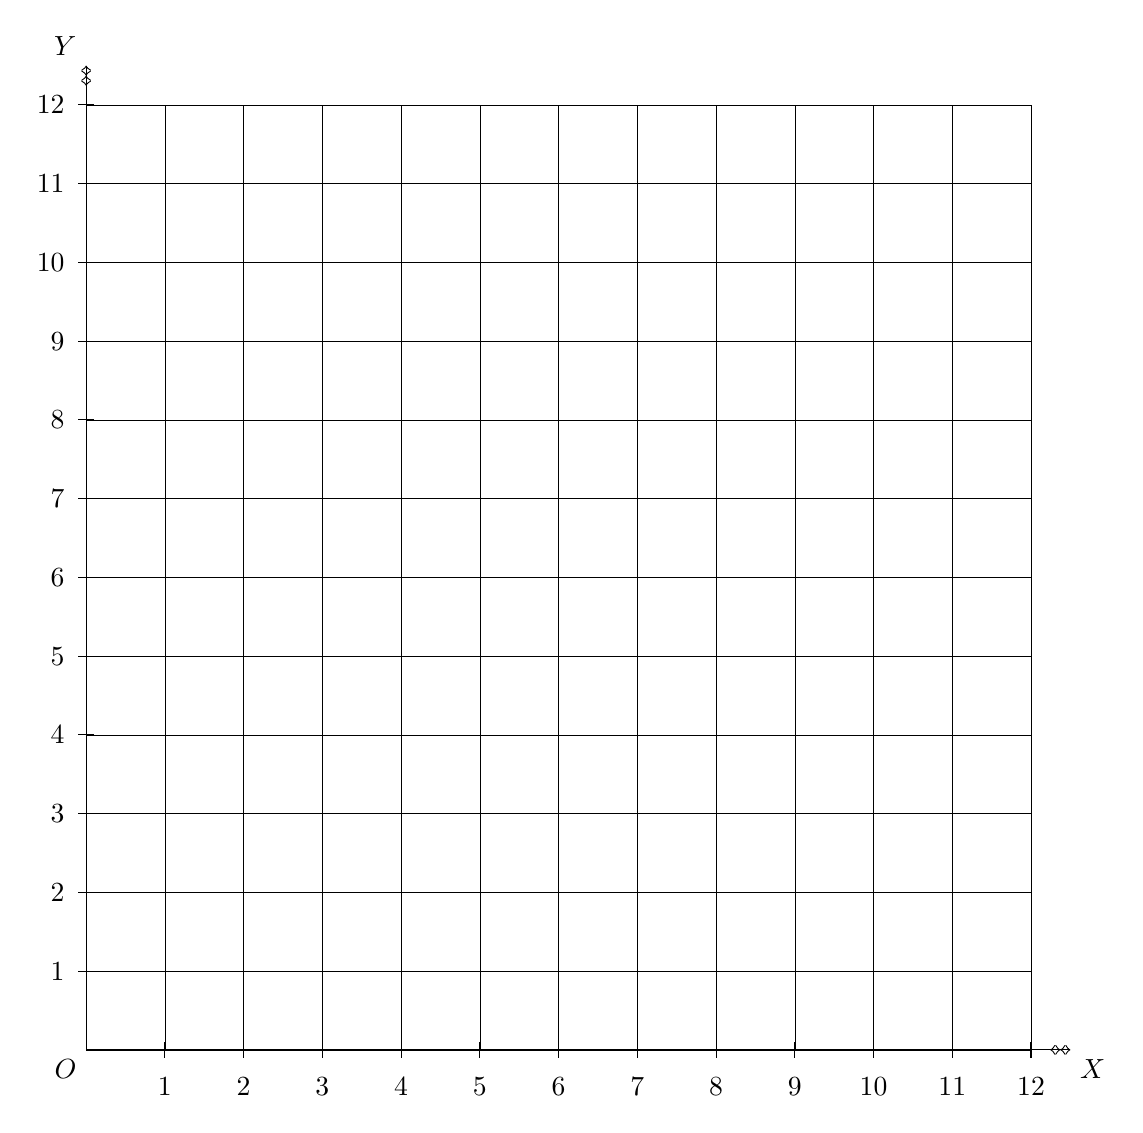
\begin{tikzpicture}
		\draw[help lines,black] (0,0) grid (12,12);
        \draw [] (0,0)--(0,0) node[below left] {$O$};
		\draw [-<><>] (0,0)--(12.5,0) node[below right] {$X$};
		\draw [-<><>] (0,0)--(0,12.5) node[above left] {$Y$};
		\foreach \i in {1,...,12}{
            \draw (\i,-0.1)--++(90:0.2) node[above=-8mm]{\i};
        }
		\foreach \i in {1,...,12}{
            \draw (0.1,\i)--++(180:0.2) node[left=0.5mm]{\i};
        }
	\end{tikzpicture}
}
\end{document}
